\clubpenalty100000000
\widowpenalty100000000
\documentclass[svgnames,12pt]{scrartcl}

\usepackage{xltxtra,polyglossia}
\usepackage{graphicx}
\usepackage[round]{natbib}
\usepackage{xcolor, color, colortbl, multirow}
\usepackage{url}
\setmainfont{Times New Roman}
\setmainlanguage{english}
\fontfamily{ptm}\selectfont

\setcitestyle{aysep={},citesep={,},notesep={:}}
\newfontfamily\hana{HAN NOM A}
\newcommand\Chinese[1]{{\hana #1}}
\newcommand\Comment[1]{\textcolor{red}{#1}}

\title{Save the Trees: Why we need tree models in linguistic reconstruction}
\author{DRAFT}
\begin{document}
\maketitle
\begin{abstract}
  \small
Scepticism against the tree model has a long tradition in historical linguistics.  Although scholars
have emphasized that the tree model and its longstanding counterpart, the wave theory, are not
necessarily incompatible, family trees are unrealistic and should be completely abandoned from
historical linguistics has always enjoyed a certain popularity. This scepticism has further
increased with recently proposed techniques for data visualization which seem to confirm that we can 
study language history without trees.  In this paper, we show that family trees are not only a
logical but also a practical necessity in linguistic reconstruction. While the logical necessity of
the tree model follows directly from the basic assumptions underlying linguistic reconstruction, the
practical necessity of the tree-model follows from its implications for a realistic modeling of
language history, which always needs to involve a before and after of events.  In order to save the
trees from the critics, we further show that the concrete arguments brought up in favor of
anachronistic wave models do not hold. In comparing the phenomenon of \emph{incomplete lineage
sorting} in biology with processes in linguistics, we show that data which does not seem to be
resolvable in trees may well be explained without turning to diffusion as an explanation.  
Since the diffusability of features varies, we further show that the failure to find the right tree
when relying on easily diffusable features does by no means imply that a tree hypothesis could never
be substantiated when using less easily diffusable feature sets.  While acknowledging that not all
aspects of language history are tree-like, and that integrated models which capture both vertical
and lateral language relations may depict language history more realistically, we show that all
models which claim that vertical language relations can be completely ignored are essentially wrong:
Either they silently still use family trees, or they only provide a static display of data and thus
fail to model temporal aspects of language history.
\end{abstract}
\section{Introduction}
All languages develop by descent with modification: linguistic material is transferred from
generation to generation of speakers, and slight modifications in pronunciation, denotation, and
grammar may sum up to changes which are so large that when two or more linguistic varieties have been
separated in some way, be it by geographical or political separation of their speakers, they may
become mutually incomprehensible. Not all linguistic material is necessarily inherited from the
parent generation. Linguistic material may easily be transferred across linguistic boundaries or
diffuse across similar speech varieties. This does, however, not change the fact that the primary
process by which languages are transmitted is the acquisition of a first language by children.
\textcolor{red}{look for ringe quote on this ringe 2002}. That largely incomprehensible and
different languages may share a common genetic origin was one of the great insights of 19th century
linguistics, and even if lateral forces of transmission may drastically change the shape of
languages, this does not invalidate the crucial role that genetic inheritance plays in language
history. 
%\Comment{slightly repeat the abstract with citations, but potentially not as verbose as we did in
Skepticism against the tree model has a long tradition in historical linguistics. Criticizing the tree model is almost as old as the tree model itself and started not long after the first scholars used evidence drawn from the early version of the comparative method to reconstruct family trees from Indo-European and its subgroups (\citealt{Celakovsky1853,Schleicher1853}, see \citealt{Geisler2013}). 

\Comment{... let's see later how to further expand this ...}

\section{Dendrophobia and Dendrophilia in the History of Linguistics}
In order to get a clearer argument of the major arguments brought up to support or to dismiss the
family tree model it is useful to have a closer look at the origins of the tree model and the
discussions that it instigated. In the following, we will give a brief overview on the historical
background on dendrophilia and dendrophobia in linguistics.

\subsection{Dendrophilia}
Although not being the first to draw language trees,\footnote{The first trees and networks depicting
language development date at least back to the 17th century (for details, see \citealt{List2016h},
\citealt{Morrison2016}, and \citealt{Sutrop2012}).} it was August Schleicher (1821-1866) who made
tree-thinking popular in linguistics. In two early papers from 1853
\citep{Schleicher1853,Schleicher1853a}, and numerous studies published thereafter (see, for example,
\citealt{Schleicher1861,Schleicher1863}), he propagated that the assumptions about language history
could be best `{illustrated by the image of a branching tree'
\citep[787]{Schleicher1853}.\footnote{Our translation, original text: `[Diese Annahmen, logisch
folgend aus den Ergebnissen der bisherigen Forschung,] lassen sich am besten unter dem Bilde eines
sich verästelnden Baumes anschaulich machen'.} Note that there was no notable influence by Darwin
here. It is more likely that Schleicher was influenced by \emph{stemmatics} (manuscript comparison,
see \citealt[8]{Hoenigswald1963}); and even today, historical linguistics has certain features that
resemble manuscript comparison much more closely than evolutionary biology. It seems that
Schleicher's enthusiasm for the drawing of language trees had quite an impact on Ernst Haeckel
(1834-1919, see \citealt{Sutrop2012}), since – as Schleicher pointed out himself
\citep[14]{Schleicher1863} – linguistic trees by then were concrete and not abstract like the one
Darwin showed in his Origins \citep{Darwin1859}.
 
Despite the seemingly radical idea to model language history as process of diversification
exclusively via branching and splitting, it is important to note that Schleicher was not a careless
proponent of tree thinking. Judging from his work we find many examples showing that he was aware of
potential problems resulting from the tree model. Thus, in his open letter to Haeckel, Schleicher,
taking Latin and its descendants as an example, explicitly pointed to problems of language mixing
which he compared to plant hybrids in biology, identifying it as a second factor leading to
differentiation \citep[18]{Schleicher1863}. 
In his earlier work, he mentioned language contact and
borrowing of linguistic features explicitly as a process characteristic for language history \citep[6]{Schleicher1861}, emphasizing the importance of
distinguishing borrowed from inherited traits in language classification \citep[30]{Schleicher1848}.
Following up the analogy with species evolution, Schleicher also pointed to the problem of finding
sharp borders between languages, dialects, and speech varieties (`Sprache, Dialekt, Mundarten und
Untermundarten' in the original), which finds a counter-part in the distinction between species and
individuals \citep[21]{Schleicher1863}. Especially this last point clearly reflects
that Schleicher did not exclusively think that
language splits were a product of abrupt separation of speakers, and that he was aware of the
idealizing aspect of the \emph{Stammbaum}.
\subsection{Dendrophobia}
Schleicher's tree-thinking, however, did not last very long in the world of historical linguistics.
By the beginning of the 1870s Hugo Schuchardt (1842-1927) and Johannes Schmidt (1843-1901) published
critical views, claiming that vertical descent was all what language evolution is about
\citep{Schmidt1872,Schuchardt1870}. While Schmidt remained very vague in his criticism, Schuchardt
was concrete and observant in his criticisms, especially pointing to the problem of borrowing
between very closely related languages, which might deeply blur the phylogenetic signal: 

\begin{quote}
\small We connect the branches and twigs of the family tree with countless horizontal lines and it ceases
to be a tree. \citep[9]{Schuchardt1870}\footnote{Our translation, original text: `Wir verbinden die
Äste und Zweige des Stammbaums durch zahllose horizontale Linien, und er hört auf ein Stammbaum zu
sein.'} 
\end{quote}

While Schuchardt's observations were based on his deep knowledge of the Romance languages, Schmidt
drew his conclusions from a thorough investigation of shared homologous words in the major branches
of Indo-European. What he found were patterns of words that were in a strong \emph{patchy
distribution} (see \citealt{List2014a}), that is, showing many gaps across the languages, with only
a few (if at all) patterns that could be found across all languages. One seemingly surprising fact
was, for example, that Greek and Sanskrit shared about 39\% of cognates (according to Schmidt's
count, see \citealt{Geisler2013}), Greek and Latin shared 53\%, but Latin and Sanskrit only 8\%.
Assuming that Greek and Latin had a common ancestor, Schmidt found it very difficult to explain how
the similarities between the two languages with Sanskrit could be so different
\citep[24]{Schmidt1872}. Furthermore, this pattern of patchy distributions seemed to be repeated in
all branches of Indo-European that Schmidt compared in his investigation. Schmidt thus concluded: 

\begin{quote}
     \small No matter how we look at it, as long as we stick to the assumption that today's languages
     originated from their common proto-language via multiple furcation, we will never be able to
     explain all facts in a scientifically adequate way. \citep[17]{Schmidt1872}\footnote{Our
     translation, original text: `Man mag sich also drehen und wenden wie man will, so lange man an
     der Anschauung fest hält, dass die in historisches Zeit erscheinenden sprachen durch merfache
     Gabelungen aus der Ursprache hervorgegangen seien,d.h. so lange man einen stammbaum der
     indogermanischen Sprachen annimmt, wird man nie dazu gelangen alle die hier in frage stehenden
     tatsachen wissenschaftlich zu erklären.'} 
\end{quote}

Schmidt, however, did not stop with this conclusion but proposed another model of language
divergence instead of the family tree model:

\begin{quote} \small I want to replace [the tree] by the image of a wave that spreads out from the
     center in concentric circles becoming weaker and weaker the farther they get away from the
     center. \citep[27]{Schmidt1872}\footnote{Our translation, original text: `Ich möchte an seine
     \emph{[des Baumes]} stelle das bild der welle setzen, welche sich in concentrischen mit der
     entfernung vom mittelpunkte immer schwächer werdenden ringen ausbreitet.'} 
\end{quote}

Ever since then, this new model, the
so-called \emph{wave theory} (\emph{Wellentheorie} in German) has been vividly discussed in articles and textbooks in
in historical linguistics, sometimes being promoted as the missing complement of Schleicher's
\emph{Stammbaumtheorie}, sometimes being treated as its more realistic alternative.
Although most historical linguists would probably assume that they have a clear understanding of
what the wave theory is, it has led to a significant amount of confusion, not only among linguists
themselves, but also among those who are not primarily trained in historical linguistics.
This confusion is not only reflected in the discussions between dendrophilists and dendrophobists,
but also in the various attempts that have been made to visualize the waves.
While Schmidt did
not give a visualization in his book from 1872, he gave one 3 years later \citep[199]{Schmidt1875},
as shown in Figure \ref{fig:schmidt1875} along with an English translation.
It is difficult to interprete this Figure, not only due to the quality, but also due to its
structure, which is hard to understand intuitively: It displays languages in a pie-chart-like
diagram in a quasi-geographic space. No information regarding ancestral states of the languages is
given, and no temporal dynamics are shown. Being quasi-geographic, quasi-quantitative, and
quasi-structured, the visualization is hard to understand, and the famous waves themselves are the
least thing one thinks about when inspecting it. Schmidt does not seem to ignore that evolution has
a time dimension, but he seems to deliberately neglect it when drawing his waves.
Other scholars, like \citet[93]{Hirt1905}, \citet[316]{Bloomfield1933}, \citet[134]{Meillet1908}, or
\citet[174]{Bonfante1931}, proposed similar and alternative ways to visualize Schmidt's waves (see
\citealt{Geisler2013}). In contrast to the language trees which – after Schleicher's initial rather
``realistic" tree drawings – quickly began to be schematized in historical linguistics, the correct
way to draw a wave has remained a mysterium up to today.

\begin{figure}[htb]
\centering
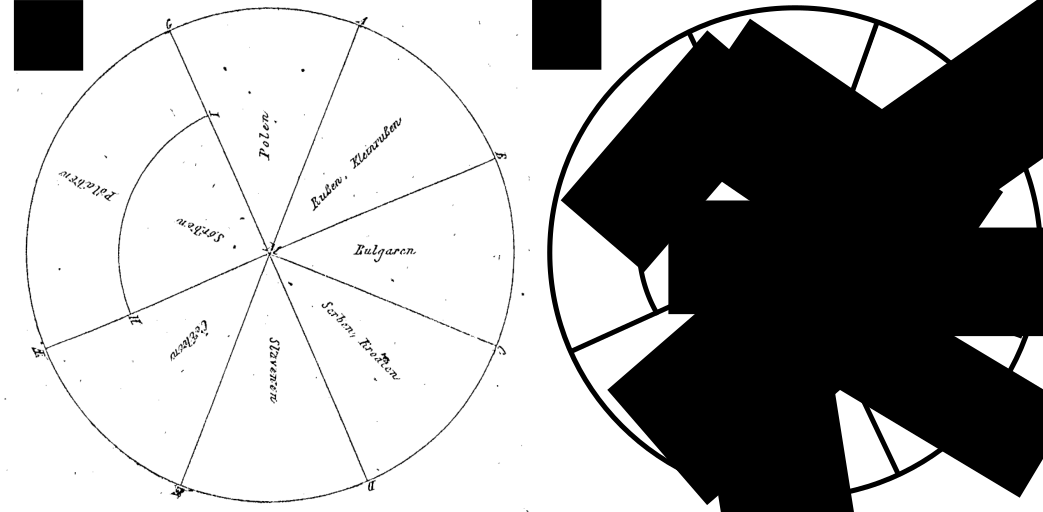
\includegraphics[width=0.75\textwidth]{images/schmidt-1875.pdf}
\caption{Schmidt's Wave Theory. A: Schmidt's visualization of the Wave Theory from 1875. B: English
translation.}
\label{fig:schmidt1875}
\end{figure}

Visualization problems, however, cannot be taken to discredit a theory, although they may reflect
problems of internal coherence. \citet[118-120]{Geisler2013} distinguish three different kinds of
criticisms that have been raised against the family model (and in favor of the wave theory): (1)
practicabily problems, (2) plausibility problems, and (3) adequacy problems. Practicability
problems refer to the problems in applying the tree model to analyse a given set of languages. In
the critics they may be reflected in conflicting evidence, as reflected in Schmidt's work mentioned
above \citep{Schmidt1872}. Plausibility problems refer to the realism of the family tree model and
are reflected in obvious simplifications provoked by the tree model. They are reflected in critics
emphasizing that languages do not necessarily split abruptly but slowly diverge accompanied by
complex waves of diffusion \citep{Schuchardt1870,Schmidt1872}. Adequacy refers to the purpose of
writing language history in historical linguistics. Critics complain that family trees break down
all vivid aspects that are substantial for the diversification of a language family to processes of
vertical descent. 
 
While all three types of criticism have been brought up against the family tree model, it is clear
their theoretical strength differs drastically. Refusing a model for practicality reasons is
straightforward, but it cannot be used to prove that a model is wrong or inadequate.  Surprisingly,
especially the work by Johannes Schmidt reflects a high degree of ignorance regarding the
epistemological limits and the temporary status of knowledge in historical linguistics. Being not
able to find evidence for a tree in a given dataset is no proof that the family tree model is wrong,
in the same way as the inability to distinguish borrowed from inherited traits the further one goes
back in time can be considered as proof against the existence of tree-like divergence of languages.
Stronger arguments against the family tree model were therefore those that challenged its
plausibility, with respect to the presumed split-process by which languages diverge, or its
adequacy, with respect to its ability to provide a full picture of language history in all its
complexity.
 
As mentioned earlier, Schleicher was well aware of the most problematic aspects of the tree
model, namely the possibility of hybridization and an often gradient as opposed to an abrupt
transition underlying language divergence, and he deliberately ignored these aspects in the family
tree model, giving a strict preference to divergence and vertical inheritance. Proponents of the
wave theory, on the other hand, are much less clear about the different processes they seek to
model. Do wave-like processes of language change reflect borrowing among closely related languages,
or are they intended to reflect language change in general? While \citet{Schuchardt1870} seems to distinguish
the two, pointing to \emph{horizontal lines} (`{horizontale Linien}') that make a network out of a
tree, \citet{Schmidt1872} is much less explicit, although he often invokes the idea of gradual
transitions between language borders \citep[200]{Schmidt1875}, thus emphasizing the gradualness of
diversification rather than the interference of vertical and lateral processes in language change.
Given the diversity of opinions and the lack of concreteness, it is
difficult to determine a core theory to which scholars refer when mentioning the Wave theory, and
while some see the wave theory as the horizontal counterpart of the family tree \citep[74]{Baxter2006a},
others see the wave theory as a theory explaining linguistic divergence \citep[188-191]{Campbell1999}

\subsection{The New Debate on Trees and Waves}
Along with the ``quantitative turn" in historical linguistics \citep[209f]{List2014d}, the debate on
trees and waves was revived. Had most textbooks treated both models as a complementary view on
\emph{external language history}\footnote{External language history is here used in the sense of
\citet{Gabelentz1891} who distinguishes it from internal language history pointing to different
stages of one and the same language.} \citep{Lehmann1992,Anttila1972} or as treating two completely
different aspects of language change \citep{Campbell1999}, more and more linguists now began to 
discuss the models as opposing perspectives \citep{Francois2015}. One reason for the revival of the
discussion was the prevalence for trees in early phylogenetic studies in historical linguistics
\citep{Gray2003,Atkinson2006,Ringe2002,Pagel2009}. Had both trees and waves been playing a less
prominent role for a long time,\footnote{Even Morris Swadesh never used his lexicostatistic method to
produce family trees. Instead, he published a map on ``interrelationships of American Indian
languages" that comes closer to an interpretation in terms of the wave theory
\citep[23]{Swadesh1959}.} biological methods for phylogenetic reconstruction applied to large
linguistic datasets now offered a quick and much more transparent way to display language data in a
tree diagram than the classical method of identifying shared innovations.
Only a few years after the first large phylogenetic trees of languages were reconstructed, new
visualization techniques for splits networks (most of them based on the NeighborNet algorithm,
\citealt{Bryant2004}), as provided by the SplitsTree software package \citep{Huson1998} offered
scholars a fresh view on conflicts in their data which was often propagated as a reconciliation of
tree and wave theory \citep{Hamed2006,Heggarty2010,McMahon2005}.


\section{Theoretical and Practical Necessity of the Tree Model}
\Comment{as in the longer abstract above, but of course, more verbose, with more references,
basically, this is, what was before labelled as:
\begin{itemize}
    \item The tree model as a logical consequence of the comparative method
\end{itemize}
Part written by M + G}
\section{The Advantages of the Tree Model}
\Comment{Here, it would be the parts mentioned not in he abstract, but in the first draft, with
arguments by G}

\section{Saving the Trees from the Critics}
Given the logical necessity to allow for divergence, a specific part of language history can be
modeled with help of a tree if specific processes like recombination (hybridization, creolization)
can be excluded. That such a tree model does not necessarily represent all aspects of language
history is obvious, and even the strongest tree proponents would not deny it. Whether the amount
of inheritance versus borrowing in language history is as low as it was supposed for biology, where
tree critics have labeled the tree of life as the ``tree of one percent'' \citep{Dagan2006} is an
interesting question worth being pursued further. Given that we know that language varieties can
diverge to such an extent that they loose mutual intelligibility, however, necessitates a model for
language history which handles divergence and splits of lineages. How these splits proceed in the
end, whether they are best viewed as multifurcations after the split of a larger dialect continuum
in several parts, or as bifurcations, depends on our insights into the language family under
investigation and into the processes of external language change in general. 
\subsection{Not Seeing the Tree for the Forest}
When scholars point out that a given datasets lacks tree-like signal, or that the tree-like signal
for the subgrouping of a given language family is not strong, they often take this as direct
evidence for large-scale language contact or linkage scenarios \citep{Ross1988}.  This, however, is
by no means the only explanation for reticulations in datasets, and many other reasons why a given
data selection may fail to reveal a tree (see the general overview in
\citealt[44-66]{Morrison2011}). The most obvious and in cases of large dataset most frequent reason
are erroneous codings which occur especially in those cases where the data has not been thoroughly
checked by the experts in the field \citep{Geisler2010}, or where automatic analyses have introduced
a strong bias. Another obvious reason is the selection of the data. Commonalities in sound change
patterns and grammatical features, for example, often do not represent true shared innovations but
independent development, and especially for sound changes it is often very hard to distinguish
between synapomorphy and homplasy \citep[182f]{Chacon2015}, which is exacerbated by the fact that
the majority of sound change patterns are extremely common, while rare sound changes are often very
difficult to prove. Apart from borrowing, dialect differentiation, data coding, and homoplasy,
another often overlooked cause of reticulations in the data is the process of \emph{incomplete
lineage sorting} \citep{Galtier2008}. Incomplete lineage sorting is a well-known process in
biology, during which polymorphisms in the ancestral lineages are inherited by the descendent
languages when rapid divergence occurs \citep{Rogers2014}. Incomplete lineage sorting can explain 
why 30\% of the genes in a Gorilla's genome are more similar to the human genome or to the
Chimpanzee genome although human and chimpanzee are the closest relatives \citep{Scally2012}. 
In a recent study, \citet{List2016h} proposed that incomplete lineage sorting may likewise occur in
language history, given  
the multiple sources of polymorphisms in language change, ranging from near synonymy of lexical
items via suppletive paradigms to word derivation.
Apart from these language-internal factors of polymorphisms which may be inherited across lineages,
before they are
later randomly resolved, an further factor not mentioned by \citet{List2016h} is variation in the
population of speakers, or sociolinguistic variation, which, in contrast to biology, where every
organism has only one gene for each function, may even occur in one and the same speaker. 
The process of incomplete lineage sorting is further illustrated in Figure \ref{fig:ils}, where the
two aspects, namely sociolinguistic variation, and language-internal variation are contrasted. Note
that in neither of the cases we even need to invoke neither strong language contact nor situations
of large scale diffusion in dialect networks. Both patterns are perfectly compatible with a ``social
split" situation as invoked by \citet{Francois2015}, although they are based on fully resolved
bifurcating trees. This shows that supposed reticulations in the data, or lack of tree-like signal
in the data do not necessarily prove the absence of tree-like patterns of divergence. They rather
expose the weakness of our methods to find the tree in the forest of individual histories of
linguistic traits.  

\begin{figure}[htb]
  \centering
  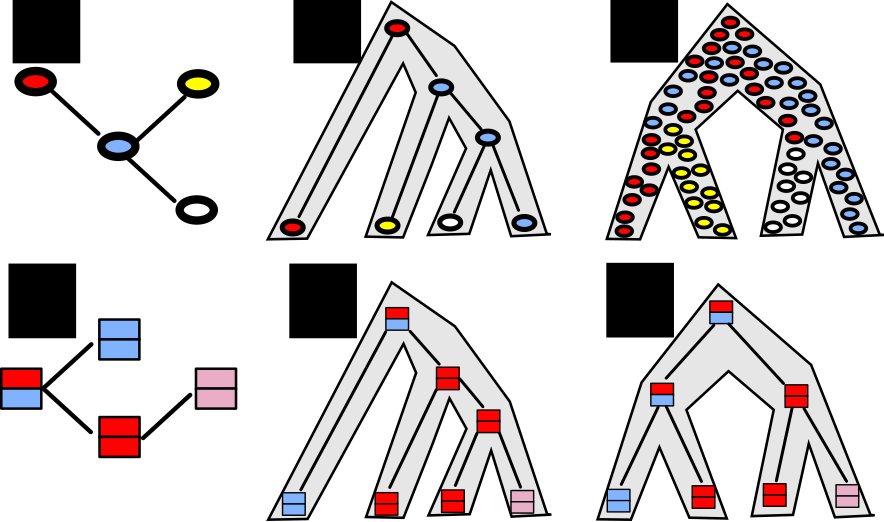
\includegraphics[width=\textwidth]{images/ils.pdf}
  \caption{Incomplete lineage sorting due to sociolinguistic (A-C) and linguistic variation (D-F) and its impact
  on phylogenetic reconstruction and genetic subgrouping. A shows a pattern of know directional
  evolution of a character (e.g., a sound change pattern), and B shows one of the most parsimonious
  trees resulting from the pattern. C shows an alternative pattern by assuming that the blue
  character already evolved in the ancestral language where it was used as a variant along with the
  original red character. Since the variation already occurred at the time of the ancestral
  languages, it was inherited in the two descendant languages from which the character further
  developed. As a result, another tree topology can be reconstructed. D gives an example for a
  process of paradigm leveling, and E and F show two possible equally parsimonious scenarios
  invoking different tree topologies each.}
  \label{fig:ils}
\end{figure}

\subsection{Diffusability of Features}
\Comment{Here, G formulates the optimistic message that we can RANK our features and do not need to
be as pessimistic as the glottometric-people}
\subsection{Limitations of Sound Correspondences}
\Comment{Here, G further follows up the last part in the abstract on sound correspondences}
\section{Conclusion}
\Comment{following passage from long abstract probably useful}
While acknowledging that not all aspects of language history are tree-like, and that integrated
models which capture both vertical and lateral language relations may depict language history more
realistically, we show that all models which claim that vertical language relations can be
completely ignored are essentially wrong. Either they silently still use family trees, or they only
provide a static display of data and thus fail to model temporal aspects of language history.







\bibliographystyle{plainnat}
\bibliography{bibliography,example}

\end{document}

